\documentclass[12pt,journal,compsoc]{IEEEtran}

\usepackage[portuguese]{babel}
\usepackage[utf8]{inputenc}
\usepackage{graphicx}
\usepackage[font=small,labelfont=bf]{caption}
\usepackage{breakurl}
\usepackage{color}

\begin{document}

\title{Otimização de Análise Estática de Código com SonarQube e Eclipse}
\author{
  Daniel~M.~Assis
  \IEEEcompsocitemizethanks{
    \IEEEcompsocthanksitem Daniel M. Assis (daniel.medeiros.assis@gmail.com)
  }
}

\IEEEcompsoctitleabstractindextext{%
\begin{abstract}
Uma das formas mais preditivas de garantir qualidade em software é através da análise estática de código-fonte. Contudo, um desafio constante tem sido a definição da forma mais efetiva de tirar proveito desta análise. Este artigo apresenta um método prático, que faz uso de conceitos e ferramentas, para atingir eficiência na melhoria da qualidade de código.
\end{abstract}
\begin{IEEEkeywords}
Static Code Analysis, SonarQube, Eclipse, Enterprise, CheckStyle, FindBugs, PMD
\end{IEEEkeywords}}

\maketitle

\IEEEdisplaynotcompsoctitleabstractindextext
\IEEEpeerreviewmaketitle

\section{Introdução}

\IEEEPARstart{P}{o}r uma série de fatores, nem sempre o código-fonte de um software acaba sendo escrito da melhor forma. Frente a isto, ferramentas como o SonarQube\cite{sonarqube} (previamente chamado "Sonar"\cite{sonar_sonarqube})  atuam, apoiando, dentre outros aspectos, na análise do código. Tal análise (\emph{estática}, no sentido que verifica a forma como os artefatos estão escritos) sugere correções em pontos específicos, o que resulta diretamente em melhoria de qualidade. 

A \emph{análise estática de código} é, portanto, um conceito que faz uso de ferramentas para avaliar o código-fonte em relação a um conjunto de regras pré-estabelecidas que determinam a melhor forma de escrita. O objetivo da análise é evidenciar problemas, para que possam ser corrigidos com o máximo de foco, resultando em maior eficiência no processo de melhoria de qualidade. Contudo, a análise de código feita tardiamente no ciclo de vida do desenvolvimento de software pode ser pouco produtiva - e tal análise precisa fazer o melhor uso das ferramentas disponíveis para ser realmente eficiente. 

Este artigo irá apresentar um método e ferramentas para otimização da aplicação da análise estática de código em relação ao procedimento tradicional, de forma a aumentar a eficiência no processo de melhoria de qualidade e, consequentemente, refletir na redução dos custos com manutenção.


\section{Análise preditiva}

A análise estática de código pode ser feita em diferentes momentos no ciclo de vida de desenvolvimento, e geralmente não é feita de forma preditiva: o código é analisado e corrigido apenas depois de já ter sido versionado (o que significa que já pode estar em homologação ou produção). Este processo pode ser ilustrado conforme segue:

\begin{figure}[ht!]
\centering
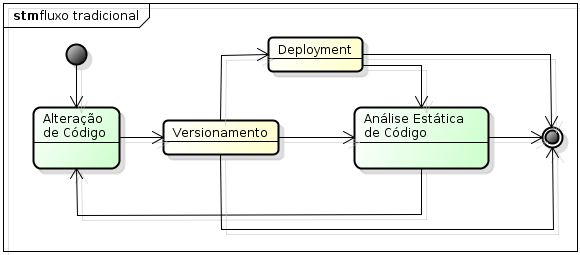
\includegraphics[width=0.5\textwidth]{img/flow_before}
\caption{análise estática de código a posteriori}
\label{flow_before}
\end{figure}

Esse fluxo apresenta algumas desvantagens:

\begin{itemize}
\item a análise somente ocorre depois do código já ter sido versionado, de forma que o mesmo código precisa ser \emph{revisitado} para ajustes e novo versionamento e/ou deployment; 
\item a pessoa que corrige uma análise pode não ser a mesma que implementou originalmente, o que pode aumentar a complexidade da correção, ocasionando atrasos;
\item não há garantias que uma análise estática de código acabe resultando em melhoria efetiva no código-fonte analisado  
\end{itemize}

Sabe-se que quanto mais cedo um problema é encontrado no código, mais barato é para corrigí-lo, em escala exponencial\cite{software_engineering_economics}. Com base neste conceito, uma \emph{verificação antecipada} da aderência do código-fonte em relação às regras no ciclo de vida do desenvolvimento traz benefícios no custo da correção de problemas (em forma de redução de tempo e recursos gastos na atividade de melhoria de código). Desta forma, propõe-se uma inversão no fluxo, de forma que a análise estática de código possa acontecer juntamente com a alteração de código e antes do versionamento. Um fluxo \emph{preditivo} é descrito abaixo:

\begin{figure}[ht!]
\centering
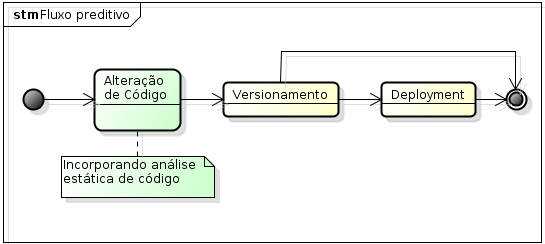
\includegraphics[width=0.5\textwidth]{img/flow_after}
\caption{Fluxo com Análise preditiva}
\label{flow_after}
\end{figure}

Esta simplificação no fluxo exige, na prática, que o desenvolvedor realize a análise estática de código (e a correção indicada) antes de versionar a modificação\cite{jamesshore_ci_attitude}. O SonarQube poderia, posteriormente, evidenciar uma estabilidade no número de violações em relação ao tempo (e com esta estabilidade observada, seria possível eliminar a prática de \emph{"enxugar gelo"}, por meio da atuação na redução efetiva de violações sem que novas violações estejam sendo adicionadas pelo ciclo de desenvolvimento em paralelo). 

Contudo, para que o desenvolvedor incorpore o trabalho de análise de código-fonte à sua rotina de forma a não impactar em sua produtividade, é preciso que as ferramentas de análise estática de código sejam o mais transparente possíveis em relação à necessidade de execução. Uma alternativa comum a ser citada poderia ser o uso da ferramenta SonarQube localmente na máquina do desenvolvedor; contudo, esta abordagem apresenta-se pouco produtiva, pois exige esforço explícito do desenvolvedor e configuração adicional externa à IDE, de forma que não é transparente quanto à sua execução \emph{(a seção "Experimento e resultados observados", deste artigo, detalha este problema por meio de um breve estudo de caso)}. Desta forma, a abordagem sugerida é a de que a própria IDE indique as violações no código conforme estejam sendo escritas. Para isto, a IDE precisa fazer uso de plugins que validem o código-fonte em relação às regras de qualidade assumidas pela empresa. 


\section{Ferramentas e Métodos}

O SonarQube é uma ferramenta que, dentre outras funções, possui plugins capazes de realizar a análise estática de código por meio de um conjunto padrão de regras. Abaixo, segue uma descrição geral dos plugins mais populares para este fim:

\begin{itemize}
\item Checkstyle: verifica e valida aderência do código-fonte em relação a convenções de escrita;
\item PMD: verifica e valida a adoção de boas práticas;
\item FindBugs: verifica potenciais bugs
\end{itemize}

Estes mesmos plugins também estão disponíveis para Eclipse, que é a IDE mais popular para desenvolvimento Java\cite{java_report_2012}. 

Desta forma, objetivando a configuração da IDE que valide automaticamente o código-fonte sendo modificado com base nas regras da empresa, o processo de configuração do Eclipse para incorporar as regras do SonarQube consiste em:

\begin{itemize}
\item configurar o Eclipse para utilizar os mesmos plugins do SonarQube (FindBugs, PMD e Checkstyle); 
\item exportar as regras do SonarQube de cada um dos plugins e importar no Eclipse;
\end{itemize}

A versão do SonarQube utilizada neste trabalho é a 4.3, e a versão do Eclipse é a 4.3.2 (Kepler).
O procedimento de configuração é descrito em detalhes, abaixo.

\subsection{Exportando as regras do SonarQube}

O processo de exportação das regras do SonarQube é bastante simples e exige apenas uns poucos passos. Deve-se acessar a opção de menu "Quality Profile", escolher o "Java Profile", clicar no link "Permalinks" do breadcrumb de Coding rules e então exportar as regras. As figuras ilustram este fluxo de navegação.

\begin{figure}[ht!]
\centering
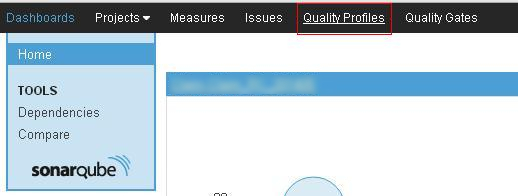
\includegraphics[width=0.5\textwidth]{img/sonar-step-01}
\caption{Quality Profile do SonarQube}
\label{sonar-step-01}
\end{figure} 

\begin{figure}[ht!]
\centering
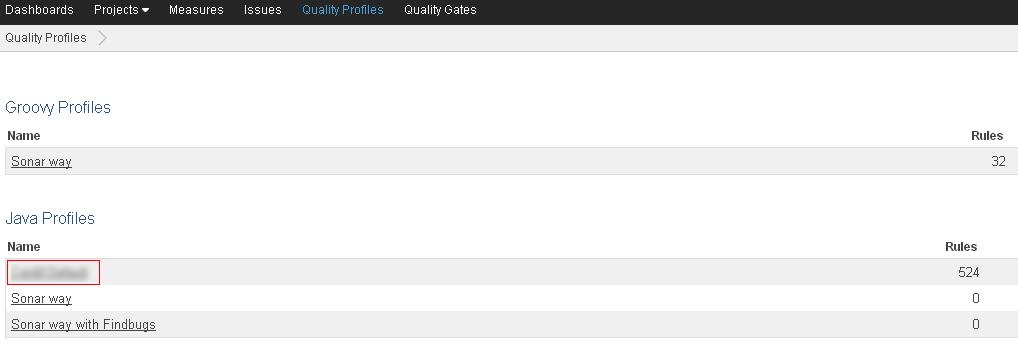
\includegraphics[width=0.5\textwidth]{img/sonar-step-02}
\caption{Selecionando o Java Profile}
\label{sonar-step-02}
\end{figure} 

\begin{figure}[ht!]
\centering
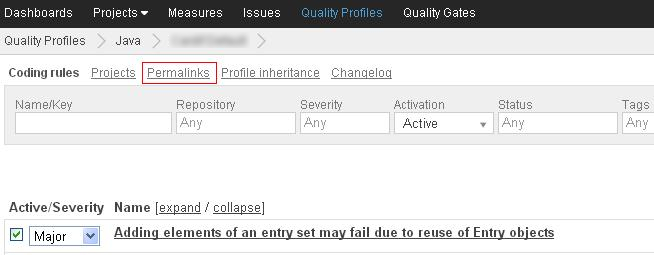
\includegraphics[width=0.5\textwidth]{img/sonar-step-03}
\caption{Permalinks do breadcrumb "Coding Rules"}
\label{sonar-step-03}
\end{figure} 

\begin{figure}[ht!]
\centering
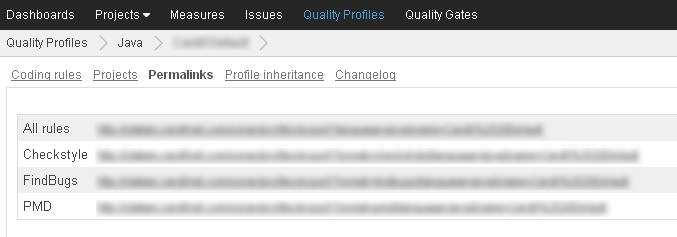
\includegraphics[width=0.5\textwidth]{img/sonar-step-04}
\caption{Lista de regras por plugin de análise estática de código}
\label{sonar-step-04}
\end{figure} 

As regras precisam ser exportadas individualmente, para cada um dos três plugins (Checkstyle, PMD e FindBugs), em arquivos XML distintos. Tais arquivos devem ser salvos para importação posterior no Eclipse.

Por fim, considerando questões de compatibilidade de versão, ainda é preciso realizar duas simples substituições no conteúdo do XML exportado do PMD. São elas:

\begin{itemize}
\item "rulesets/" por "rulesets/java/"
\item "controversial.xml/UnusedModifier" por "unusedcode.xml/UnusedModifier"
\end{itemize}


\subsection{Configurando FindBugs no Eclipse}

O primeiro passo é acessar o menu do Eclipse: "Help/Install New Software", para adicionar o repositório do plugin do FindBugs\cite{FindBugs_eclipse_plugin}:

\begin{figure}[ht!]
\centering
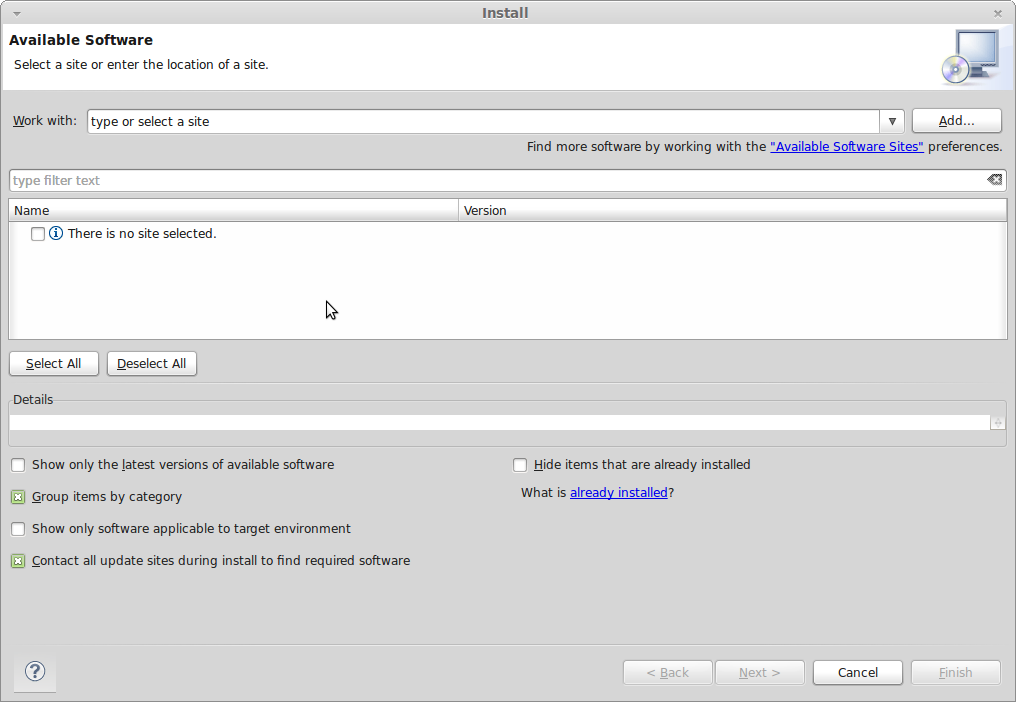
\includegraphics[width=0.5\textwidth]{img/eclipse-findbugs-01}
\caption{Install New Software}
\label{eclipse-findbugs-01}
\end{figure}

Após isto, clique em "Add" para adicionar o repositório do FindBugs "http://findbugs.cs.umd.edu/eclipse/":

\begin{figure}[ht!]
\centering
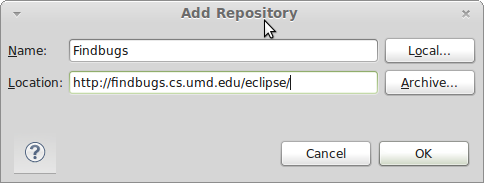
\includegraphics[width=0.5\textwidth]{img/eclipse-findbugs-02}
\caption{Adicionando repositório}
\label{eclipse-findbugs-02}
\end{figure} 

Então, selecione o plugin do FindBugs para instalação, e clique em "Next". Após isto, confirme os detalhes da instalação, clicando em "Next".

\begin{figure}[ht!]
\centering
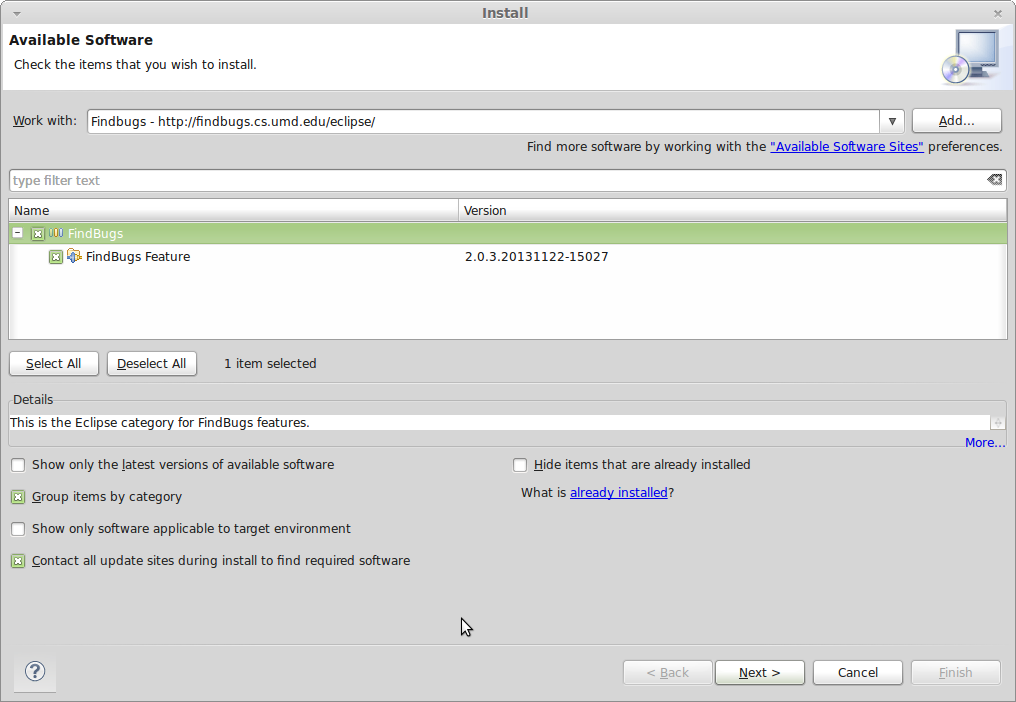
\includegraphics[width=0.5\textwidth]{img/eclipse-findbugs-03}
\caption{Selecionando FindBugs para instalação}
\label{eclipse-findbugs-03}
\end{figure} 

\begin{figure}[ht!]
\centering
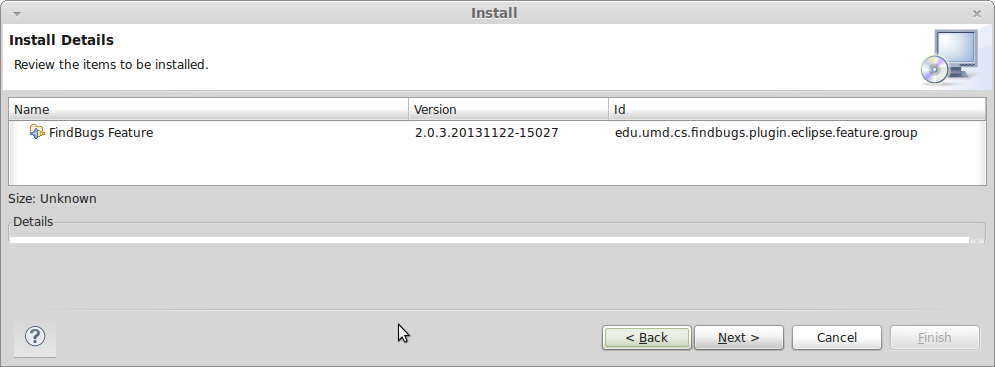
\includegraphics[width=0.5\textwidth]{img/eclipse-findbugs-04}
\caption{Confirmando detalhes da instalação}
\label{eclipse-findbugs-04}
\end{figure} 

A próxima etapa é aceitar os termos da licença de instalação. Basta clicar em "I accept the terms of the license agreement", e então em "Finish"

\begin{figure}[ht!]
\centering
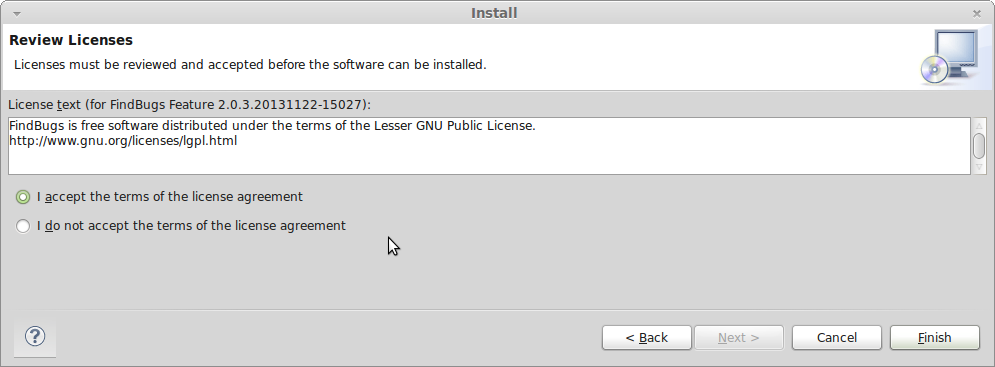
\includegraphics[width=0.5\textwidth]{img/eclipse-findbugs-05}
\caption{Aceitando termos de licença}
\label{eclipse-findbugs-05}
\end{figure} 

Durante a execução do processo de instalação do plugin, o Eclipse exibirá uma alerta informando que o conteúdo nao está assinado. Basta confirmar com "OK" para finalizar a instalação. Então, reinicie o Eclipse.

\begin{figure}[ht!]
\centering
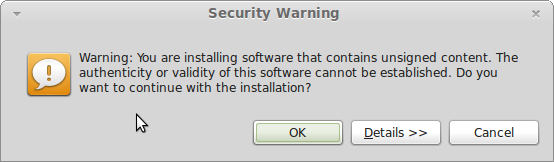
\includegraphics[width=0.5\textwidth]{img/eclipse-findbugs-06}
\caption{Aceitando conteúdo não-assinado}
\label{eclipse-findbugs-06}
\end{figure} 

Após a instalação do plugin, é preciso configurá-lo e importar as regras do SonarQube para uso. Para isto:

\begin{itemize}
\item acesse a opção do menu do Eclipse "Window/Preferences", opção "Java/FindBugs"
\item na aba "Reporter Configuration", em "Minimum rank to Report", selecione "20"
\item na aba "Reporter Configuration", em "Reported (visible) bug categories", selecione todas as opções
\item na aba "Reporter Configuration", em "Minimum Confidence to Report", selecione "Medium"
\item na aba "Filter Files", em "Include Filter Files", clique em "Add" e selecione o arquivo XML do FindBugs previamente exportado pelo SonarQube
\item na aba "Detector Configuration", selecione o checkbox "Show hidden detectors" e então marque todos os checkboxes do grid
\end{itemize}

\begin{figure}[ht!]
\centering
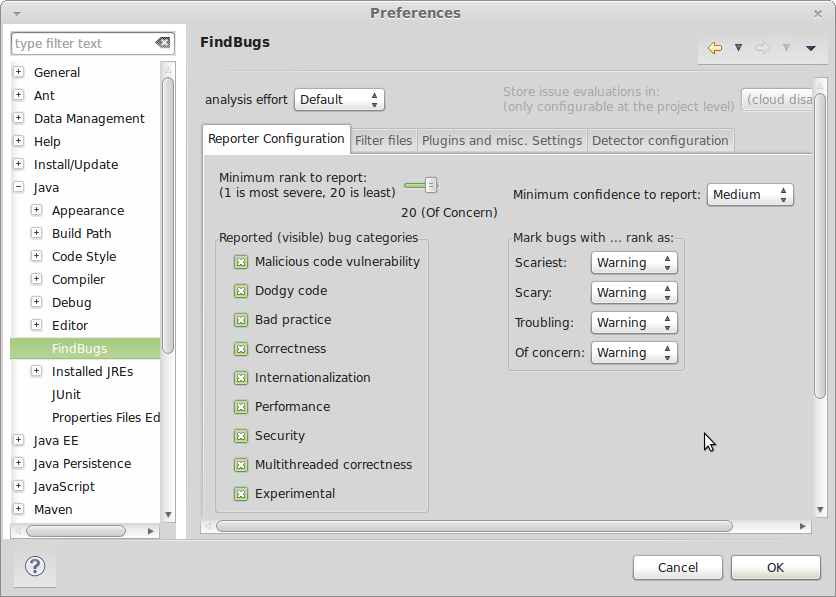
\includegraphics[width=0.5\textwidth]{img/eclipse-findbugs-07}
\caption{Configuração da aba "Reporter Configuration" do FindBugs}
\label{eclipse-findbugs-07}
\end{figure} 

\begin{figure}[ht!]
\centering
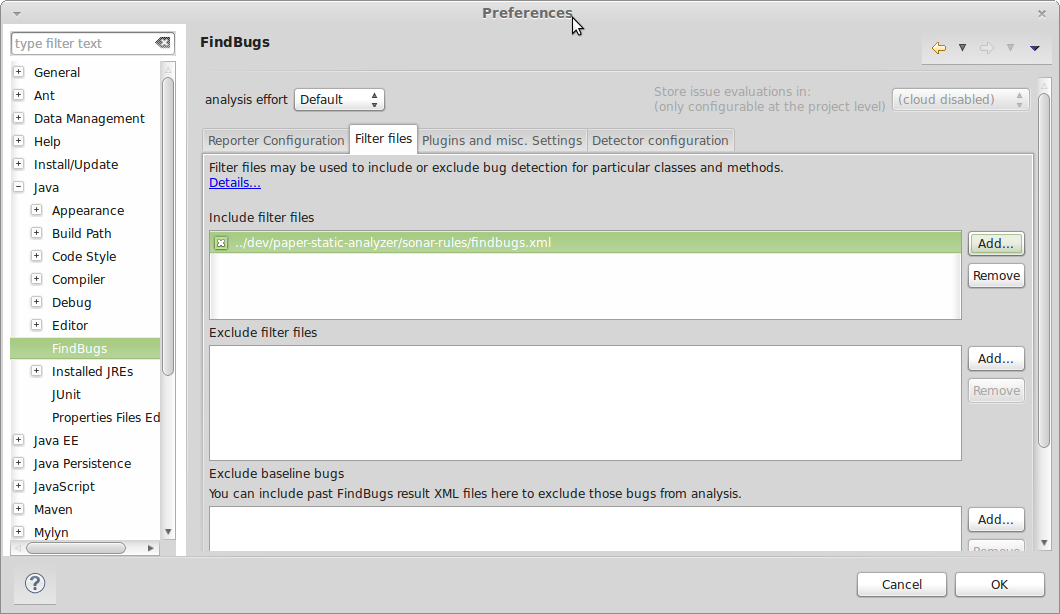
\includegraphics[width=0.5\textwidth]{img/eclipse-findbugs-08}
\caption{Configuração da aba "Filter Files" do FindBugs}
\label{eclipse-findbugs-08}
\end{figure} 

\begin{figure}[ht!]
\centering
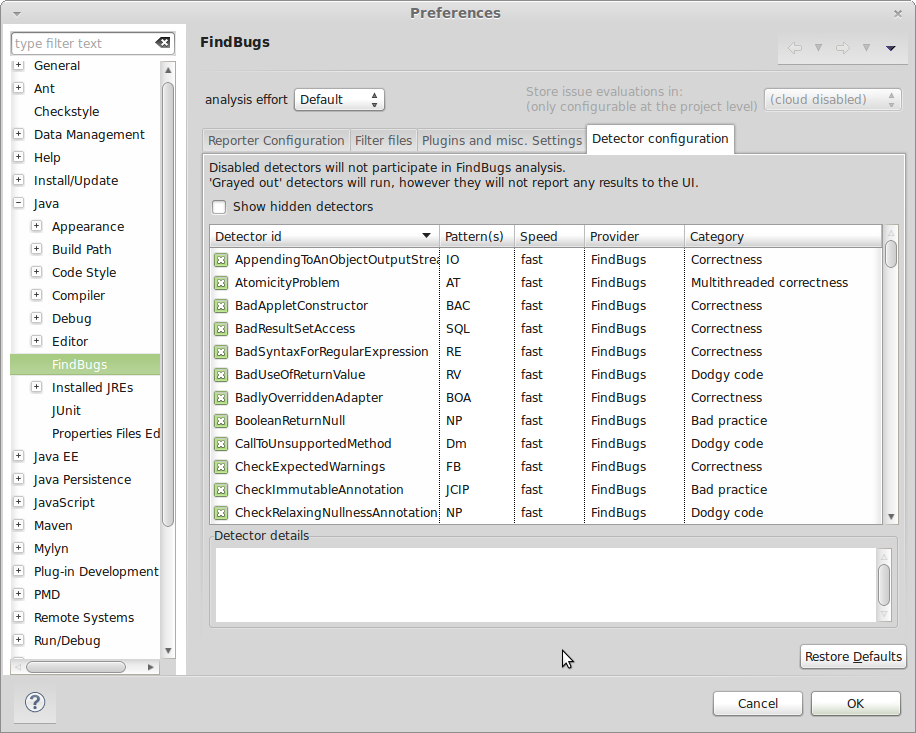
\includegraphics[width=0.5\textwidth]{img/eclipse-findbugs-08b}
\caption{Configuração da aba "Detector Configuration" do FindBugs}
\label{eclipse-findbugs-08b}
\end{figure} 

Agora, a IDE consegue validar o código-fonte utilizando as regras do FindBugs. Para isto, clique com o botão direito sobre qualquer classe, pacote ou projeto, e então em "Find Bugs/Find Bugs". Uma imagem de um bug ficará visível em linhas não-conformes, e uma descrição do bug permitirá sua correção. 

Alternadamente, é possível garantir que a validação seja realizada toda vez que uma classe for salva, através da marcação do checkbox "Run automatically", acessada pelas propriedades do projeto, opção "FindBugs".

\begin{figure}[ht!]
\centering
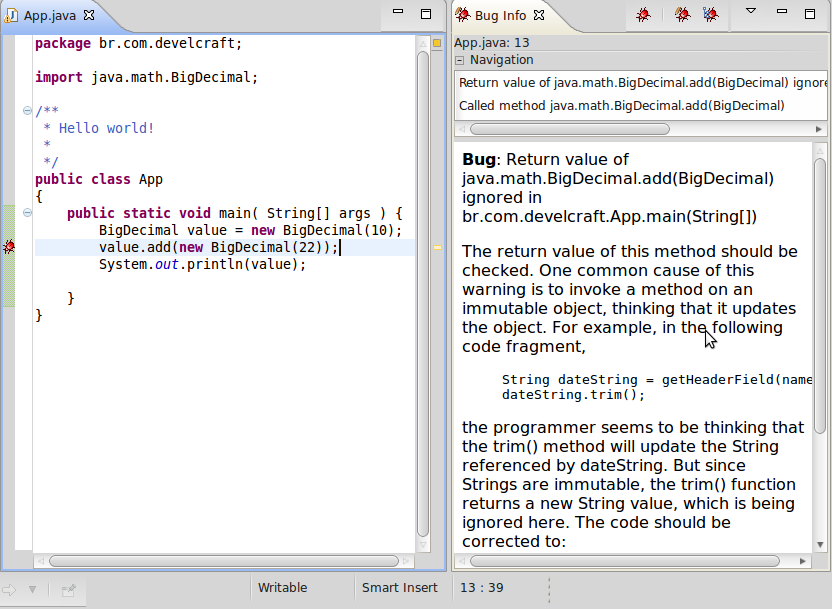
\includegraphics[width=0.5\textwidth]{img/eclipse-findbugs-09}
\caption{Interface do Eclipse após identificação de bug pelo FindBugs}
\label{eclipse-findbugs-09}
\end{figure} 


\subsection{Configurando PMD no Eclipse}

A instalação do plugin PMD\cite{pmd} segue o processo análogo à instalação do plugin FindBugs, de forma que não será novamente descrito. Apenas observam-se as seguintes especificidades:

\begin{itemize}
\item O repositório do PMD é "http://sourceforge.net/projects/pmd/
files/pmd-eclipse/update-site/";
\item O plugin a ser instalado é o "PMD for Eclipse 4".
\end{itemize}
  
Em relação à configuração do plugin, acesse o menu "Window/Preferences", opção "PMD/Rule Configuration", e siga os passos:

\begin{itemize}
\item Apague todas as regras;
\item Importe o arquivo previamente exportado pelo SonarQube, pela opção "Import Rule Set".
\end{itemize}

\begin{figure}[ht!]
\centering
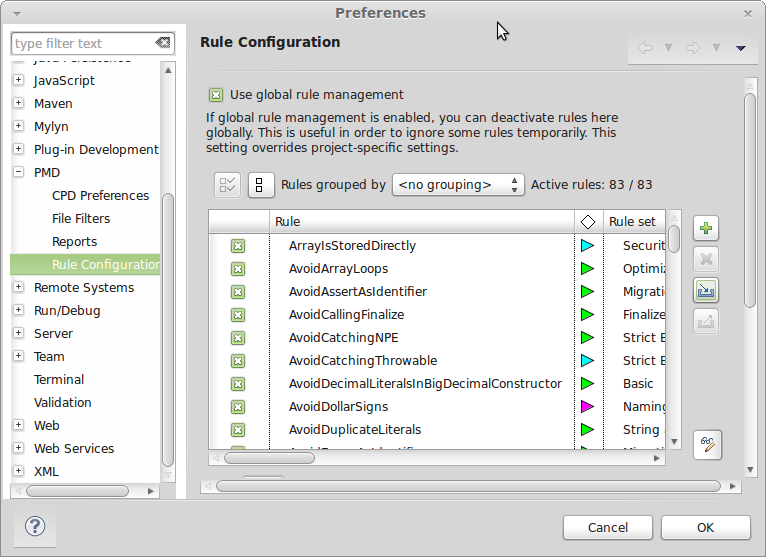
\includegraphics[width=0.5\textwidth]{img/eclipse-pmd-01}
\caption{Tela de configuração de regras do plugin PMD após importação das regras do SonarQube}
\label{eclipse-pmd-01}
\end{figure}

Agora, a IDE consegue validar o código-fonte utilizando as regras do PMD. Para isto, clique com o botão direito sobre qualquer classe, pacote ou projeto e então em "PMD/Check Code". Alternadamente, é possível garantir que a validação seja realizada toda vez que uma classe for salva, através da marcação do checkbox "Check code after saving", acessada pelo menu "Window/Preferences", opção "PMD", campo "General Options".

\begin{figure}[ht!]
\centering
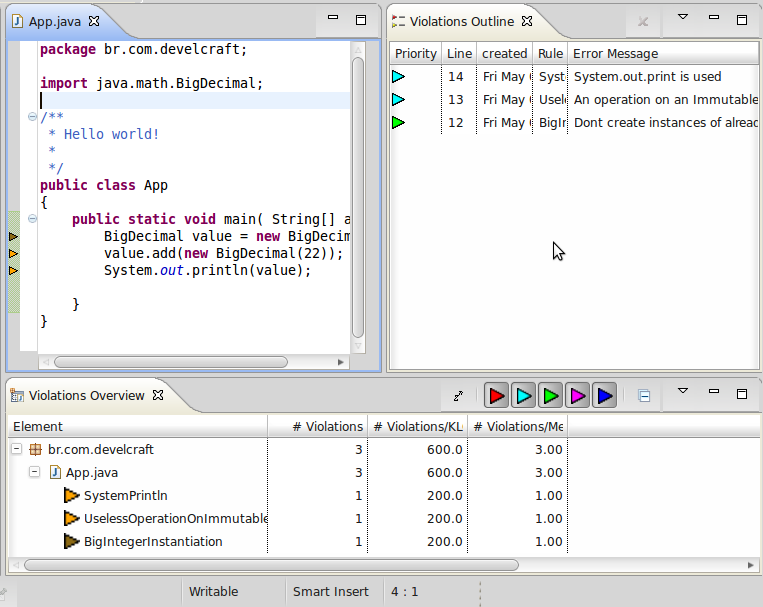
\includegraphics[width=0.5\textwidth]{img/eclipse-pmd-02}
\caption{Validação de regras pelo plugin PMD}
\label{eclipse-pmd-02}
\end{figure}

 
\subsection{Configurando Checkstyle no Eclipse}

A instalação do plugin Checkstyle\cite{checkstyle_eclipse_plugin} segue o processo análogo à instalação dos plugins FindBugs e PMD, de forma que não será novamente descrito. Apenas observam-se as seguintes especificidades:

\begin{itemize}
\item O repositório do Checkstyle é "http://eclipse-cs.sf.net/update";
\item Os artefatos a serem instalados são "Checkstyle" e "Extension for eclipse-cs plugin with additional Checks".
\end{itemize}
  
Em relação à configuração do plugin, acesse o menu "Window/Preferences", opção "Checkstyle", e siga os passos:

\begin{itemize}
\item Clique em "New", e na janela que se abre, informe o campo "Name". Na mesma janela, clique em "Import" e selecione o arquivo XML do Checkstyle exportado pelo SonarQube. Confirme com "OK"; 
\item No Grid "Global Check Configurations", selecione o Check Configuration recém-criado e clique em "Set as Default". Observe que um ícone de confirmação aparece na coluna "Default" para este item.
\end{itemize}

\begin{figure}[ht!]
\centering
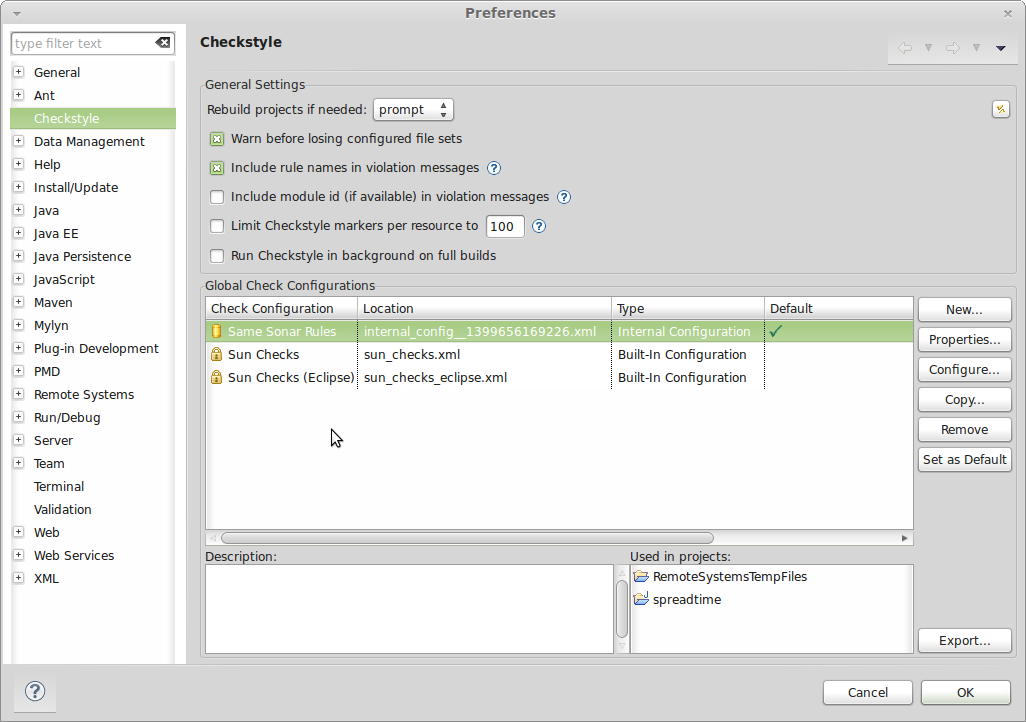
\includegraphics[width=0.5\textwidth]{img/eclipse-checkstyle-01}
\caption{Tela de configuração de regras do plugin Checkstyle após importação das regras do SonarQube}
\label{eclipse-checkstyle-01}
\end{figure}

Agora, a IDE consegue validar o código-fonte utilizando as regras do Checkstyle. Para isto, clique com o botão direito sobre qualquer classe, pacote ou projeto e então em "Checkstyle/Check Code with Checkstyle". Alternadamente, é possível garantir que a validação seja realizada toda vez que uma classe for salva: para isto, clique com o botão direito no projeto, e então em "Checkstyle/Activate Checkstyle".

\begin{figure}[ht!]
\centering
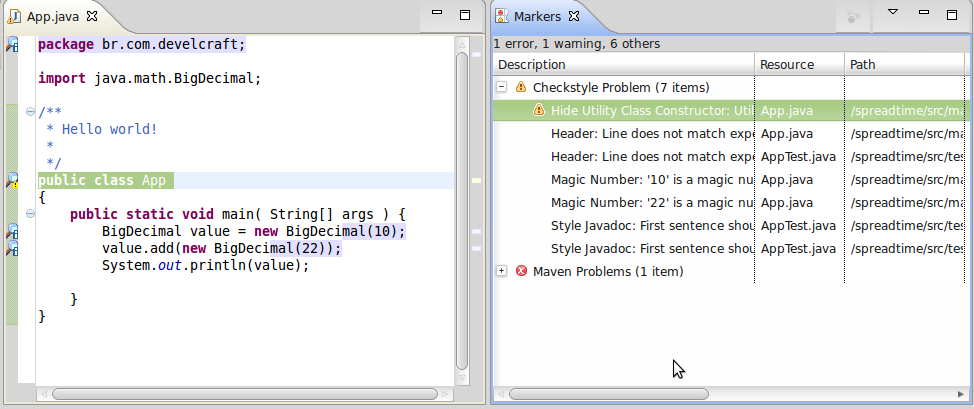
\includegraphics[width=0.5\textwidth]{img/eclipse-checkstyle-02}
\caption{Validação de regras pelo plugin Checkstyle}
\label{eclipse-checkstyle-02}
\end{figure}


\section{Experimento e resultados observados}

Como forma de validar o conceito aqui proposto, considerando tempo de identificação de violações em código-fonte e recursos consumidos pela máquina, o seguinte método Java foi criado para servir como objeto de análise:

\begingroup
\fontsize{9pt}{10pt}\selectfont
\begin{verbatim}
public BigDecimal sum()
{
    BigDecimal value = new BigDecimal(10);
    value.add(new BigDecimal(22));
    System.out.println(value);
    return value;
}
\end{verbatim}
\endgroup

Este método possui uma série de violações de diferentes níveis de criticidade, dentre elas: 

\begin{itemize}
\item uso injustificado de System.out.println;
\item má-utilização de objeto imutável (o método "add" do BigDecimal não adiciona o valor no próprio objeto - como poderia ser esperado - e sim retorna uma nova instância com a soma);
\item formatação do bloco (a chave de abertura do corpo do método não está na mesma linha da assinatura do método);
\end{itemize}

De forma a analisar violações neste código, foram aplicadas duas abordagens:

\begin{itemize}
\item Validação pelo uso de plugins corretamente configurados na IDE: a identificação de violações foi instantânea, e não foi observado aumento do consumo de memória no processo da IDE;
\item Validação sem plugins: foi preciso executar o SonarQube contra o código sendo alterado para verificar as violações. Após configuração do projeto para uso pelo SonarQube (criação e correta configuração do arquivo sonar-project.properties no diretório do projeto), os passos necessários foram: iniciar o processo do SonarQube, executar o sonar-runner no diretório do projeto (para coleta de métricas e atualização da base de dados do SonarQube), acessar a interface Web do SonarQube, e verificar as violações. O tempo observado nestas etapas levou alguns minutos e observou-se aumento de consumo de memória (criação de processo local do SonarQube). \end{itemize}


\section{Considerações Gerais}

De forma geral, as configurações dos plugins foram realizadas num nível de preferências (que é um nível mais abrangente do que o nível de configuração de projetos). Contudo, cada um dos três plugins também podem ser configurados no nível de propriedades de projeto. Quando não descrito especificamente nos passos deste artigo, recomenda-se sempre realizar as configurações no nível de preferências, e utilizar o nível de projeto apenas para configurações desejadas que sejam específicas para um dado projeto.

O método aqui proposto foi parcialmente reproduzido na IDE IntelliJ, apresentando melhores resultados que o Eclipse em relação a aspectos como integração com plugins, facilidade de configuração e estabilidade. O trabalho não foi conclusivo no sentido em que nem todos os testes foram realizados, mas sugerem potencial de maior produtividade com base nos aspectos acima citados. Desta forma, uma melhor avaliação do uso do IntelliJ é sugerida como forma a otimizar ainda mais o método e ferramentas propostos neste artigo.


\section{Conclusão}

Este artigo procurou demonstrar a forma como a análise estática de código é comumente empregada em termos de processo e ferramentas, e propor um método que faz melhor uso deste conceito, apoiado em  ferramentas apropriadas e visando redução em tempo e custo. Uma oportunidade de extensão deste trabalho é a de considerar o uso de ferramentas para integração contínua (tais como Jenkins\cite{jenkins} e Maven\cite{maven}), para realizar a verificação automatizada do emprego do método aqui proposto.

\section*{Agradecimentos}

Agradecimentos a Wender~F.~Andrade, Mario~L.~B.~C.~Gomes, Marcos~Oliveira, Helton~Ribeiro e Pedro~Leão pelo refinamento de conceitos, pelo print screen das telas do SonarQube e pela revisão deste artigo.


\bibliographystyle{IEEEtran}
\bibliography{paper-static-analyzer}

\end{document}

